\chapter{Linked Lists}
\label{ch:linkedlist}

\newcommand{\lecnum}{10}
%\newcommand{\lectitle}{Linked Lists}
\newcommand{\lecturer}{Frank Pfenning, Rob Simmons, Andr\'e Platzer,
  Iliano Cervesato}

\chapterTAGS{aliasing, correctness, ds-invariant, linked-list, queue, safety, stack}
\maketitle

\begin{preamble}
\noindent
In this lecture we discuss the use of \emph{linked lists} to implement
the stack and queue interfaces that were introduced in the last lecture.  The
linked list implementation of stacks and queues allows us to handle
work lists of any length.
\end{preamble}

\begin{gram}[Learning Goals]
This fits as follows with respect to our learning goals:
\begin{description}
\item[Computational Thinking: ]%
  We discover that arrays contain implicit information, namely the
  indices of elements, which an be made explicit as the addresses of
  the nodes of a linked list.  We also encounter the notion of
  trade-off, as arrays and linked lists have different advantages and
  drawbacks and yet achieve similar purposes.
\item[Algorithms and Data Structures: ]%
  We explore linked lists, a data structure used pervasively in Computer
  Science, and examine some basic algorithms about them.
\item[Programming: ]%
  We see that programming algorithms for linked lists can be tricky,
  which exposes once more the power of stating and checking invariant.
  We use linked lists to implement stacks and queues.
\end{description}
\end{gram}


\section{Linked Lists}
\label{sec:linkedlist:intro}
\TAGS{linked-list}

\emph{Linked lists} are a common alternative to arrays in the
implementation of data structures.  Each item in a linked list
contains a data element of some type and a \emph{pointer} to the next
item in the list.  It is easy to insert and delete elements in a
linked list, which are not natural operations on arrays, since arrays
have a fixed size.  On the other hand access to an element in the
middle of the list is usually $O(n)$, where $n$ is the length of the
list.

An item in a linked list consists of a struct containing the data
element and a pointer to another linked list.  In C0 we have to commit
to the type of element that is stored in the linked list.  We will
refer to this data as having type \lstinline'elem', with the expectation
that there will be a type definition elsewhere telling C0 what
\lstinline'elem' is supposed to be. Keeping this in mind ensures that none
of the code actually depends on what type is chosen. These
considerations give rise to the following definition:

\begin{lstlisting}[language={[C0]C}]
struct list_node {
  elem data;
  struct list_node* next;
};
typedef struct list_node list;
\end{lstlisting}

This definition is an example of a \emph{recursive type}.  A struct of
this type contains a pointer to another struct of the same type, and
so on.  We usually use the special element of type \lstinline't*', namely
\lstinline'NULL', to indicate that we have reached the end of the list.
Sometimes (as will be the case for our use of linked lists in stacks
and queues), we can avoid the explicit use of \lstinline'NULL' and obtain
more elegant code.  The type definition is there to create the type
name \lstinline'list', which stands for \lstinline'struct list_node', so that a
pointer to a list node will be \lstinline'list*'. We could also have
written these two statements in the other order, to make better use of
the type definition:

\begin{lstlisting}[language={[C0]C}]
typedef struct list_node list;
struct list_node {
  elem data;
  list* next;
};
\end{lstlisting}

There are some restriction on recursive types.  For example,
a declaration such as
\begin{lstlisting}[language={[C0]C}]
struct infinite {
  int x;
  struct infinite next;
}
\end{lstlisting}
would be rejected by the C0 compiler because it would require an
infinite amount of space.  The general rule is that a struct can be
recursive, but the recursion must occur beneath a pointer or array
type, whose values are addresses.  This allows a finite representation
for values of the struct type.

We don't introduce any general operations on lists; let's wait and see what we
need where they are used.  Linked lists as we use them here are a
\emph{concrete type} which means we do \emph{not} construct an interface and a
layer of abstraction around them.  When we use them we know about and exploit
their precise internal structure.  This is in contrast to \emph{abstract types}
such as queues or stacks whose implementation is hidden behind an interface,
exporting only certain operations.  This limits what clients can do, but it
allows the author of a library to improve its implementation without having to
worry about breaking client code.  Concrete types are cast into concrete once
and for all.


\section{List segments}
\label{sec:linkedlist:segments}
\TAGS{ds-invariant, linked-list}

A lot of the operations we'll perform in the next few lectures are on
\emph{segments} of lists: a series of nodes starting at \emph{start}
and ending at \emph{end}.

\begin{center}
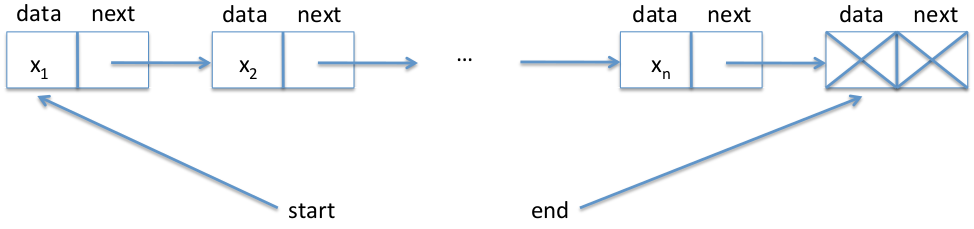
\includegraphics[width=0.99\textwidth]{img/linkedlist.png}
\end{center}
This is the familiar structure of an ``inclusive-lower,
exclusive-upper'' bound: we want to talk about the data in a series of
nodes, ignoring the data in the last node. That means that, for any
non-NULL list node pointer \lstinline'l', a segment from $l$ to $l$ is
empty (contains no data). Consider the following structure:
\begin{center}
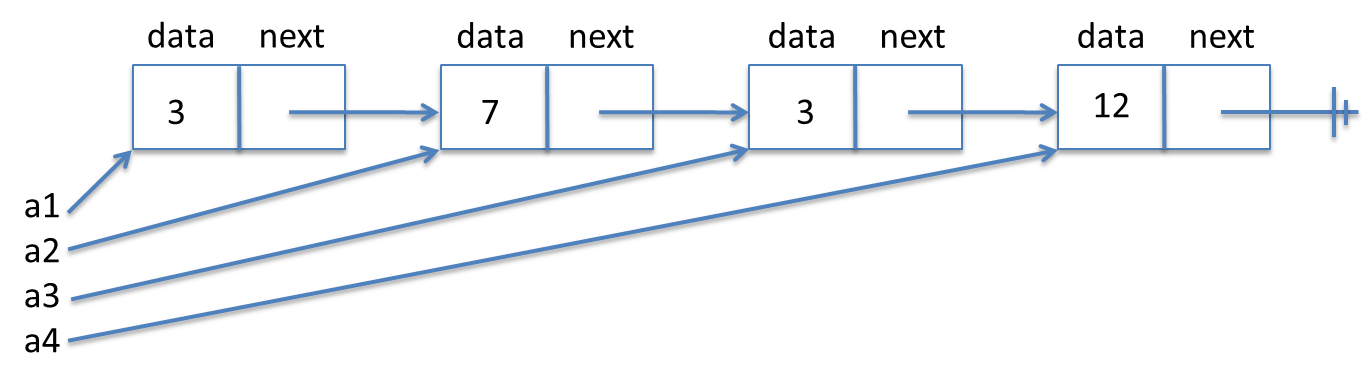
\includegraphics[width=0.95\textwidth]{img/linkedlist2.png}
\end{center}
According to our definition of segments, the data in the segment from
\emph{a1} to \emph{a4} is the sequence $3,7,3$, the data in the
segment from \emph{a2} to \emph{a3} contains the sequence $7$, and the
data in the segment from \emph{a1} to \emph{a1} is the empty
sequence. Note that, if we compare the pointers \emph{a1} and \emph{a3},
C0 will tell us they are \emph{not equal} --- even though they point to
locations that contain
the same data, \emph{a1} and \emph{a3} point to different locations in memory.

Given an inclusive beginning point \emph{start} and an exclusive
ending point \emph{end}, how can we check whether we have a segment
from \emph{start} to \emph{end}?  The simple idea is to follow
\emph{next} pointers forward from \emph{start} until we reach
\emph{end}. If we reach NULL instead of \emph{end} then we know that
we missed our desired endpoint, so that we do not have a segment. (We
also have to make sure that we say that we do not have a segment if
either \emph{start} or \emph{end} is NULL, as that is not allowed by
our definition of segments above.) We can implement this simple idea
in all sorts of ways:

\bigskip
\noindent
\textbf{Recursively:}
\begin{lstlisting}[language={[C0]C}]
bool is_segment(list* start, list* end) {
  if (start == NULL) return false;
  if (start == end) return true;
  return is_segment(start->next, end);
}
\end{lstlisting}

\medskip
\noindent
\textbf{Using a \lstinline'while' loop:}

\begin{lstlisting}[language={[C0]C}]
bool is_segment(list* start, list* end) {
  list* l = start;
  while (l != NULL) {
    if (l == end) return true;
    l = l->next;
  }
  return false;
}
\end{lstlisting}
\medskip
\noindent
\textbf{Using a \lstinline'for' loop:}

\begin{lstlisting}[language={[C0]C}]
bool is_segment(list* start, list* end) {
  for (list* p = start; p != NULL; p = p->next) {
    if (p == end) return true;
  }
  return false;
}
\end{lstlisting}
However, every one of these implementations of \lstinline'is_segment' has
the same problem: if given a circular linked-list structure, the
specification function \lstinline'is_segment' may not terminate.

It's quite possible to create structures like this, intentionally or
unintentionally. Here's how we could create a circular linked list in
Coin:
\begin{lstlisting}[language={[coin]C}]
--> list* start = alloc(list);
--> start->data = 3;
--> start->next = alloc(list);
--> start->next->data = 7;
--> start->next->next = alloc(list);
--> start->next->next->data = 3;
--> start->next->next->next = alloc(list);
--> start->next->next->next->data = 12;
--> start->next->next->next->next = start->next;
--> list* end = alloc(list);
--> end->data = 18;
--> end->next = NULL;
--> is_segment(start, end);
\end{lstlisting}
and this is what it would look like:
\begin{center}
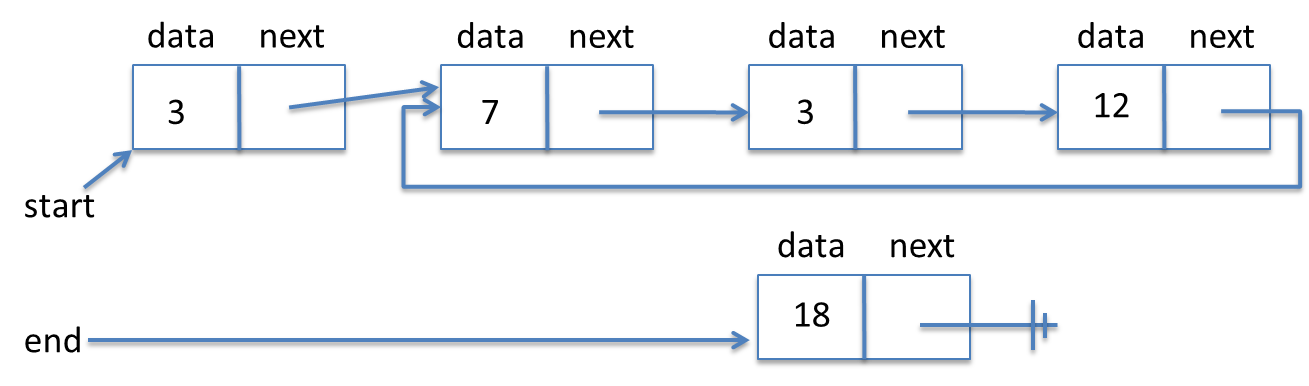
\includegraphics[width=0.9\textwidth]{img/linkedlist-circle.png}
\end{center}

\emph{Whenever possible}, our specification functions should return
\lstinline'true' or \lstinline'false' rather than not terminating or
raising an assertion violation. We do treat it as strictly necessary
that our specification functions should always be safe --- they should
never divide by zero, access an array out of bounds, or dereference a
null pointer.
%We will see how to address this problem in our next lecture.

\newpage
\section{Checking for Circularity}
\label{sec:linkedlist:circularity}
\TAGS{correctness, linked-list}

In order to make sure the \lstinline'is_segment' function correctly
handle the case of cyclic loops, let's write a function to detect
whether a list segment is cyclic. We can call this function before we
call \lstinline'is_segment', and then be confident that
\lstinline'is_segment' will always terminate.

Our cycle detection function makes use of two pointers, a \emph{fast}
and a \emph{slow} one.  Let's name them $h$ for \emph{hare} and $t$
for \emph{tortoise}.  The slow pointer $t$ traverses the list in
single steps.  Fast $h$, on the other hand, skips two elements ahead
for every step taken by $t$.  If the faster $h$ starts out ahead of
$t$ and ever reaches the slow $t$, then it must have gone in a cycle.
Let's try it on our list.  We show the state of $t$ and $h$ on every
iteration.
\begin{center}\enlargethispage{5ex}
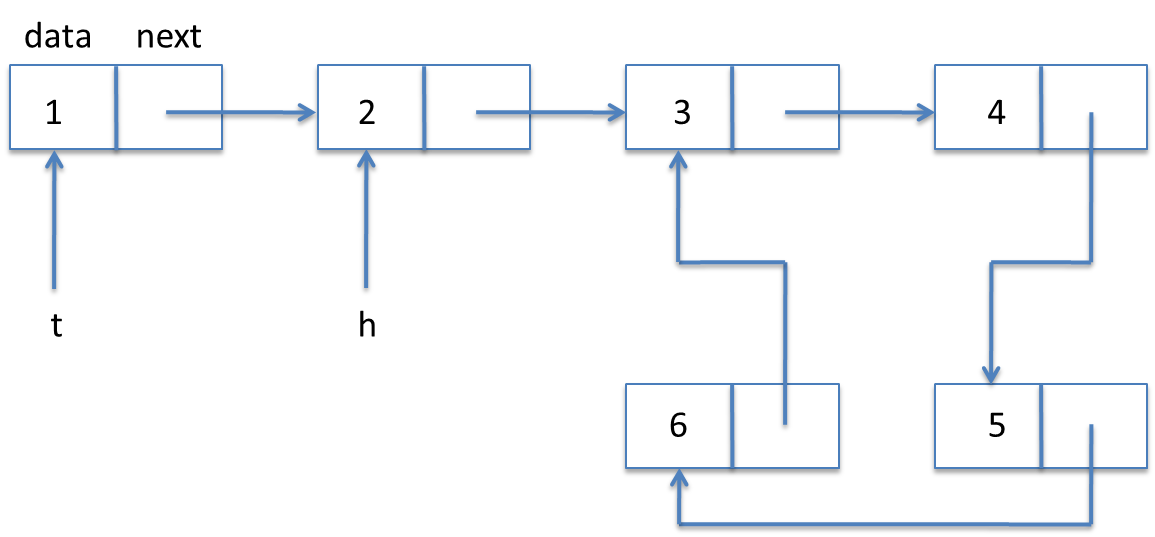
\includegraphics[width=0.75\textwidth]{img/circular2.png}
\bigskip
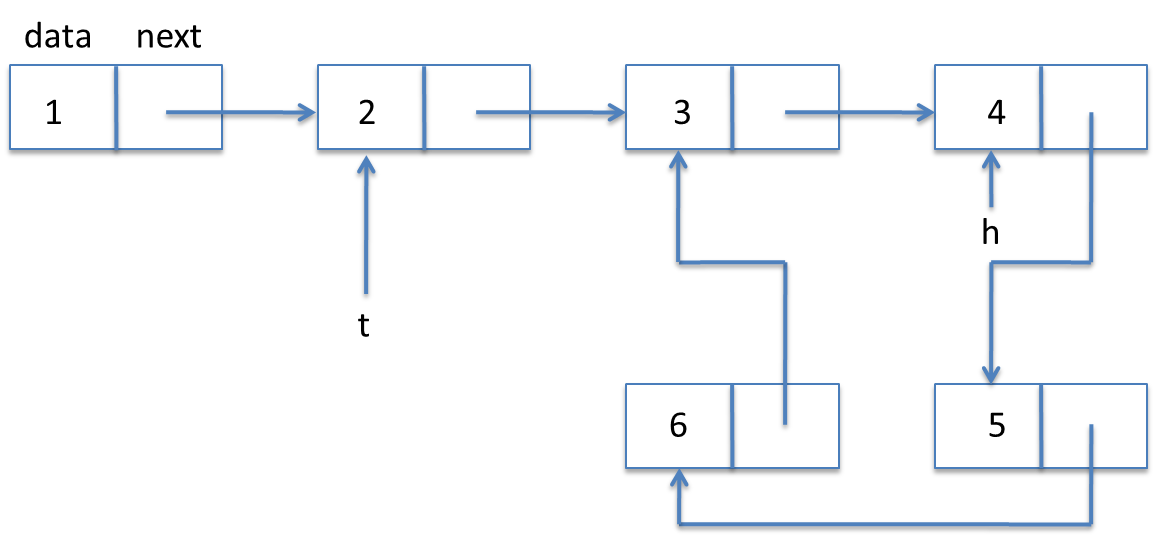
\includegraphics[width=0.75\textwidth]{img/circular3.png}
\bigskip
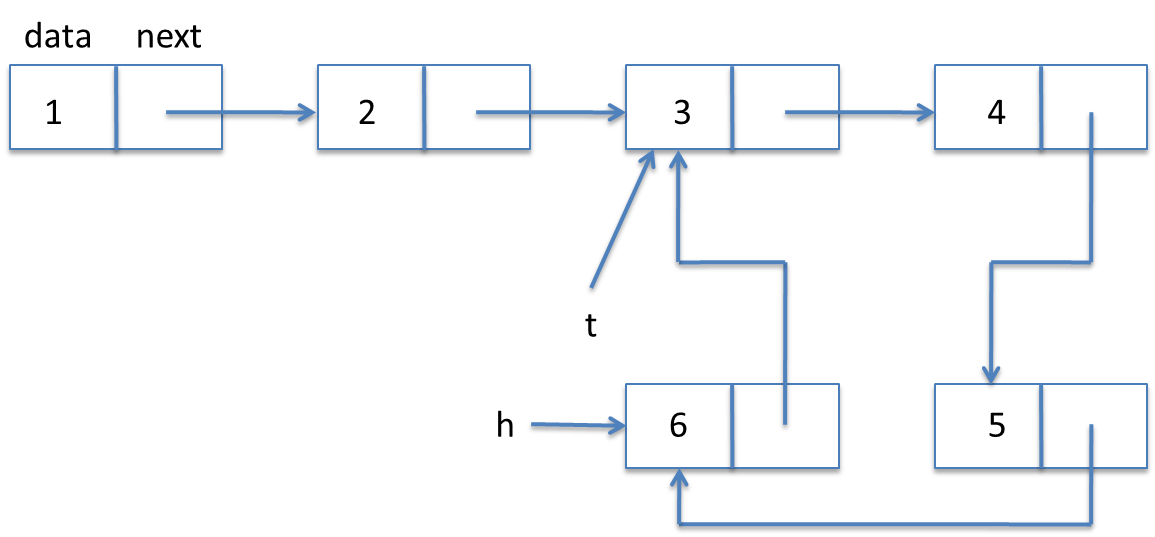
\includegraphics[width=0.75\textwidth]{img/circular4.png}
\bigskip
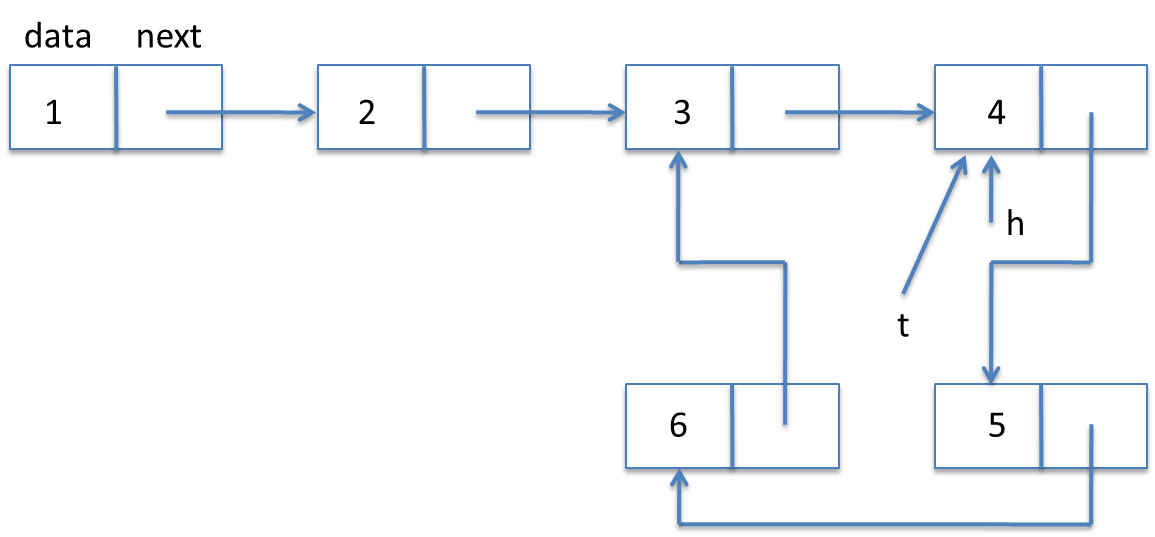
\includegraphics[width=0.75\textwidth]{img/circular5.png}
\end{center}
In code:
\begin{lstlisting}[language={[C0]C}]
bool is_acyclic(list* start) {
  if (start == NULL) return true;
  list* h = start->next;         // hare
  list* t = start;               // tortoise
  while (h != t) {
    if (h == NULL || h->next == NULL) return true;
    h = h->next->next;
    //@assert t != NULL; // faster hare hits NULL quicker
    t = t->next;
  }
  //@assert h == t;
  return false;
}
\end{lstlisting}

A few points about this code: in the condition inside the loop we
exploit the short-circuiting evaluation of the logical or `\lstinline'||''
so we only follow the next pointer for $h$ when we know it is not
\lstinline'NULL'.  Guarding against trying to dereference a \lstinline'NULL'
pointer is an extremely important consideration when writing
pointer manipulation code such as this.
The access to \lstinline'h->next' and \lstinline'h->next->next' is guarded by
the \lstinline'NULL' checks in the if statement.

%% But what about the dereference
%% of \lstinline't' in \lstinline't->next'?
%% Before you turn the page: can you figure it out?
%% \clearpage
%% One solution would be to add another if statement checking whether
%% \lstinline't==NULL'. That is unnecessarily inefficient, though, because the
%% tortoise $t$, being slower than the hare $h$, will never follow pointers
%% that the hare has not followed already successfully. In particular, they
%% cannot be \lstinline'NULL'. How do we represent this information?
%% One way would be to rely on our operational reasoning and insert an assert:
%% \begin{lstlisting}[language={[C0]C}]
%%     //@assert t != NULL; // hare is faster and hits NULL quicker
%% \end{lstlisting}
%% But as the comment indicates, it is hard to justify in logical reasoning why this assert never fails.
%% Can we achieve the same logically?
%% Yes, but while you think about how, we will first analyze the complexity of the algorithm and resolve another mystery.

%% This algorithm has complexity $O(n)$.  An easy way to see this was
%% suggested by a student in class: when there is no loop, the hare will
%% stumble over \lstinline'NULL' after $O(n/2)$ steps.  If there is a loop, then
%% consider the point when the tortoise enters the loop.  At this point,
%% the hare must already be somewhere in the loop.  Now for every step
%% the tortoise takes in the loop the hare takes two, so on every
%% iteration it comes one closer.  The hare will catch the tortoise after
%% at most half the size of the loop.  Therefore the overall complexity
%% of $O(n)$: the tortoise will not complete a full trip around the
%% loop.
%% In particular, whenever the algorithm returns \lstinline'true', it's because the hare caught the tortoise, which is an obvious cycle.
%% Yet, since, in the cyclic case, the distance between the hare and the tortoise strictly decreases in each iteration, the algorithm will correctly detect all cycles.

%% Now, where is the mystery?
%% When inspecting the \lstinline'is_acyclic' function, we are baffled why it never uses \lstinline'end'.
%% Indeed, \lstinline'is_acyclic(start, end)' correctly checks whether the \lstinline'NULL'-terminated list beginning at \lstinline'start' is cyclic, but ignores the value of \lstinline'end' entirely.
%% Hence, \lstinline'is_segment(start, end)', which calls \lstinline'is_acyclic(start, end)', will categorically return \lstinline'false' on any cyclic list even if the segment from \lstinline'start' to \lstinline'end' would still have been acyclic.

%% This is actually fine for our intended use case in stacks and queues, because we do not want them to be cyclic ever.
%% But let's fix the issue for more general uses.
%% Can you figure out how?
%% \clearpage

%% The idea is to let the hare watch out for \lstinline'end' and simply treat \lstinline'end' as yet another reason to stop iterating, just like \lstinline'NULL'.
%% If the hare passes by \lstinline'end', then the list segment from \lstinline'start' to \lstinline'end' cannot have been cyclic, because he would, otherwise, have found \lstinline'end' in his first time around the cycle already.
%% Note that the same argument would not quite work when, instead, tortoise checks for \lstinline'end', because tortoise might have just found \lstinline'end' before the hare went around the cycle already.
%% \begin{lstlisting}[language={[C0]C}]
%% bool is_acyclic(list* start, list* end) {
%%   if (start == NULL) return true;
%%   list* h = start->next;         // hare
%%   list* t = start;               // tortoise
%%   while (h != t) {
%%     if (h == NULL || h->next == NULL) return true;
%%     if (h == end || h->next == end) return true;
%%     h = h->next->next;
%%     //@assert t != NULL; // hare is faster and hits NULL quicker
%%     t = t->next;
%%   }
%%   //@assert h == t;
%%   return false;
%% }
%% \end{lstlisting}

This algorithm is a variation of what has been called the
\emph{tortoise and the hare} and is due to Floyd 1967.


%% \section{Tortoise is Never NULL}

%% Let's get back to whether we can establish why the following assertion holds by logical reasoning.
%% \begin{lstlisting}[language={[C0]C}]
%%     //@assert t != NULL; // hare is faster and hits NULL quicker
%% \end{lstlisting}
%% The loop
%% invariant \lstinline't != NULL' may come to mind, but it is hard to prove that
%% it actually is a loop invariant, because, for all we know so far, \lstinline't->next'
%% may be \lstinline'NULL' even if \lstinline't' is not.

%% The crucial loop invariant that is missing is the information that the tortoise
%% will be able to travel to the current position of the hare by following next pointers.
%% Of course, the hare will have moved on then\footnote{Isn't that Zeno paradoxical?}, but at least there is a chain of next
%% pointers from the current position of the tortoise to the current position of the hare.
%% This is represented by the following loop invariant in \lstinline'is_acyclic':
%% \begin{lstlisting}[language={[C0]C}]
%% bool is_acyclic(list* start, list* end) {
%%   if (start == NULL) return true;
%%   if (start->next == NULL) return true;
%%   list* h = start->next;         // hare
%%   list* t = start;               // tortoise

%%   while (h != t)
%%   //@loop_invariant is_segment(t, h);
%%   {
%%     if (h->next == NULL || h->next->next == NULL) return true;
%%     if (h == end || h->next == end) return true;
%%     h = h->next->next;
%%     t = t->next;
%%   }

%%   //@assert h == t;
%%   return false;
%% }
%% \end{lstlisting}
%% As an exercise, you should prove this loop invariant.
%% How would this invariant imply that $t$ is not NULL?
%% The key insight is that the loop invariant ensures that there is a linked list
%% segment from $t$ to $h$, and the loop condition ensures $t\neq h$.
%% Thus, if there is a link segment from $t$ to a different $h$, the access
%% \lstinline't->next' must work.
%% We could specify this formally by enriching the contract of \lstinline'is_segment',
%% which is what you should do as an exercise.

%% Watch out for one subtle issue, though.
%% Now the implementations and contracts of \lstinline'is_acyclic' and \lstinline'is_segment' are mutually recursive.
%% That means, with contracts enabled (\lstinline'cc0 -d'), some calls to \lstinline'is_segment' will never terminate.
%% This can be fixed by introducing a copy of \lstinline'is_segment' distinguishing cyclic from noncyclic segments.
%% The key insight is from the complexity analysis.
%% The hare and the tortoise will never be farther apart than the size of the cycle.


\section{Queues with Linked Lists}
\label{sec:linkedlist:queues}
\TAGS{correctness, ds-invariant, linked-list, queue, safety}

Here is a picture of the queue data structure the way we envision
implementing it, where we have elements $1$, $2$, and $3$ in the queue.
\begin{center}
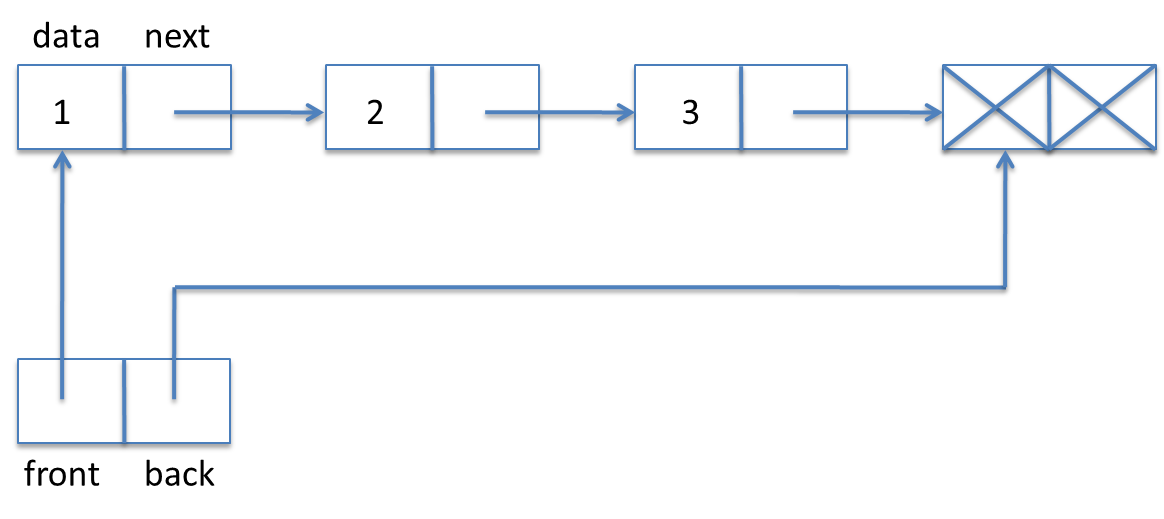
\includegraphics[width=0.85\textwidth]{img/queue1.png}
\end{center}

A queue is implemented as a struct with a \lstinline'front' and \lstinline'back'
field.  The \lstinline'front' field points to the front of the queue, the
\lstinline'back' field points to the back of the queue.  We need these two
pointers so we can efficiently access both ends of the queue, which is
necessary since dequeue (front) and enqueue (back) access different
ends of the list.

It is convenient to have the \lstinline'back' pointer point to one
element past the end of the queue.  Therefore, there is always one
extra element at the end of the queue which does not have valid data
or \lstinline'next' pointer.  We call it the \emph{dummy node} and we
have indicated it in the diagram by writing \lstinline'X'.

The above picture yields the following definition.
\begin{lstlisting}[language={[C0]C}]
typedef struct queue_header queue;
struct queue_header {
  list* front;
  list* back;
};
\end{lstlisting}
We call this a \emph{header} because it doesn't hold any elements of
the queue, just pointers to the linked list that really holds them.
The type definition allows us to use \lstinline'queue_t' as a type that
represents a \emph{pointer to a queue header}.  We define it this way
so we can hide the true implementation of queues from the client and
just call it an element of type \lstinline'queue_t'.
\begin{lstlisting}[language={[C0]C}]
typedef queue* queue_t;
\end{lstlisting}


When does a struct of this type represent a valid queue?  In fact,
whenever we define a new data type representation we should first
think about the data structure invariants.  Making these explicit is
important as we think about and write the pre- and postconditions for
functions that implement the interface.

What we need here is if we follow \lstinline'front' and then move down
the linked list we eventually arrive at \lstinline'back'.  We called
this a \emph{list segment}.  We also want both \lstinline'front' and
\lstinline'back' not to be \lstinline'NULL' so it conforms to the
picture, with one element already allocated even if the queue is
empty; the \lstinline'is_segment' function we already wrote enforces
this.
\begin{lstlisting}[language={[C0]C}]
bool is_queue(queue* Q) {
  return Q != NULL
      && is_acyclic(Q->front)
      && is_segment(Q->front, Q->back);
}
\end{lstlisting}

To check if the queue is empty we just compare its front and back.
If they are equal, the queue is empty; otherwise it is not.  We
require that we are being passed a valid queue.  Generally, when
working with a data structure, we should always require and ensure
that its invariants are satisfied in the pre- and post-conditions of
the functions that manipulate it.  Inside the function, we will
generally temporarily violate the invariants.
\begin{lstlisting}[language={[C0]C}]
bool queue_empty(queue* Q)
//@requires is_queue(Q);
{
  return Q->front == Q->back;
}
\end{lstlisting}
To obtain a new empty queue, we just allocate a list struct and point both
front and back of the new queue to this struct.  We do not initialize the list
element because its contents are irrelevant, according to our representation.
Said this, it is good practice to always initialize memory if we care about
its contents, even if it happens to be the same as the default value placed
there.
\begin{lstlisting}[language={[C0]C}]
queue* queue_new()
//@ensures is_queue(\result);
//@ensures queue_empty(\result);
{
  queue* Q = alloc(queue);    // Create header
  list* dummy = alloc(list);  // Create dummy node
  Q->front = dummy;           // Point front
  Q->back = dummy;            //   and back to dummy node
  return Q;
}
\end{lstlisting}
%% Let's take one of these lines apart.  Why does
%% \begin{lstlisting}[language={[C0]C}]
%%   queue Q = alloc(struct queue_header);
%% \end{lstlisting}
%% make sense?  According to the definition of \lstinline'alloc',
%% we might expect
%% \begin{lstlisting}[language={[C0]C}]
%%   struct queue_header* Q = alloc(struct queue_header);
%% \end{lstlisting}
%% since allocation returns the address of what we allocated.
%% Fortunately, we defined \lstinline'queue' to be a short-hand
%% for \lstinline'struct queue_header*' so all is well.

To enqueue something, that is, add a new item to the back of
the queue, we just write the data into the
extra element at the back, create a new back element, and
make sure the pointers are updated correctly.  You should draw
yourself a diagram before you write this kind of code.
Here is a before-and-after diagram for inserting \lstinline'3'
into a list.  The new or updated items are dashed in the second
diagram.
\begin{center}
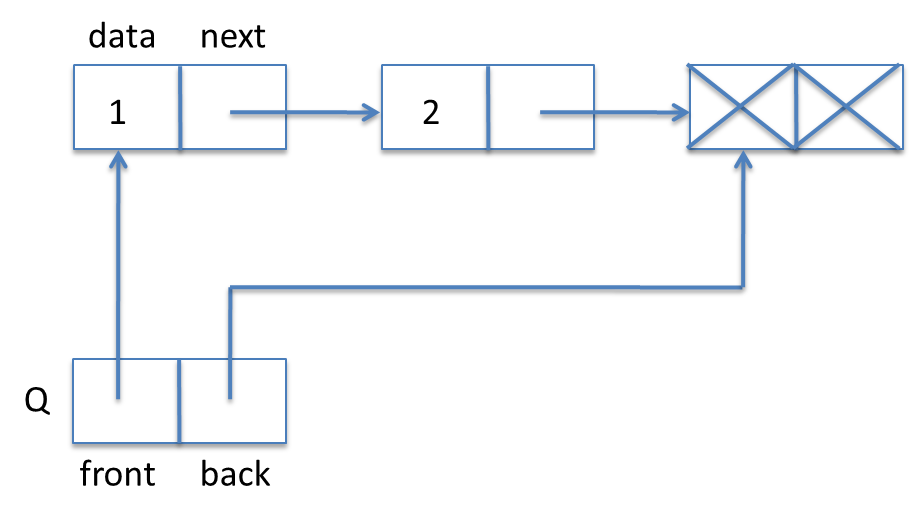
\includegraphics[width=0.67\textwidth]{img/queue2.png}\hspace*{8em}
\end{center}
\begin{center}
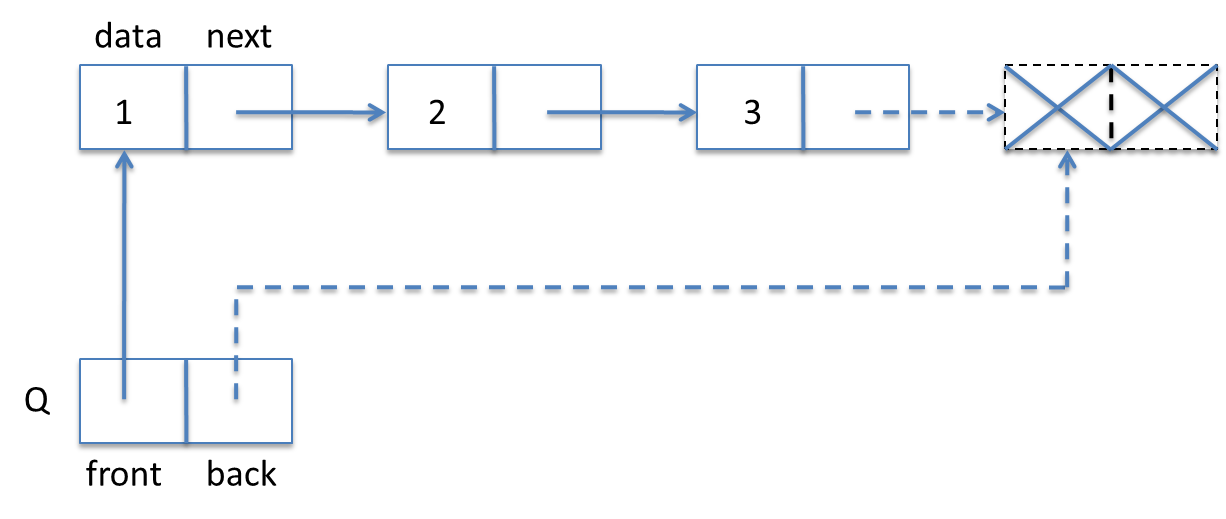
\includegraphics[width=0.9\textwidth]{img/queue3.png}
\end{center}
In code:
\begin{lstlisting}[language={[C0]C}]
void enq(queue* Q, elem x)
//@requires is_queue(Q);
//@ensures is_queue(Q);
{
  list* new_dummy = alloc(list);  // Create a new dummy node
  Q->back->data = x;              // Store x in old dummy node
  Q->back->next = new_dummy;
  Q->back = new_dummy;
}
\end{lstlisting}

Finally, we have the dequeue operation.  For that, we only need to
change the front pointer, but first we have to save the dequeued
element in a temporary variable so we can return it later.  In
diagrams:
\begin{center}
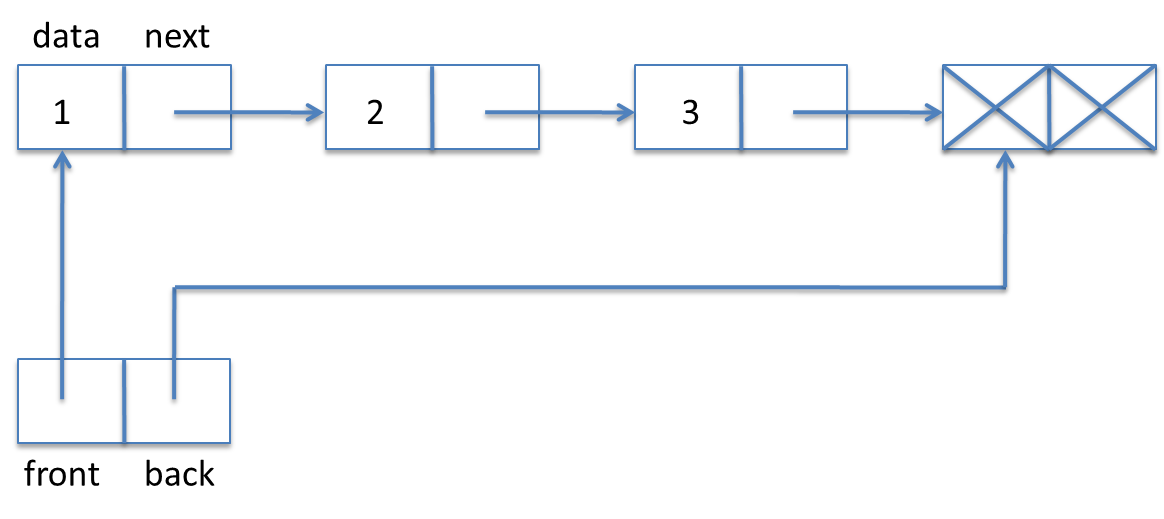
\includegraphics[width=0.85\textwidth]{img/queue1.png}
\end{center}
\begin{center}
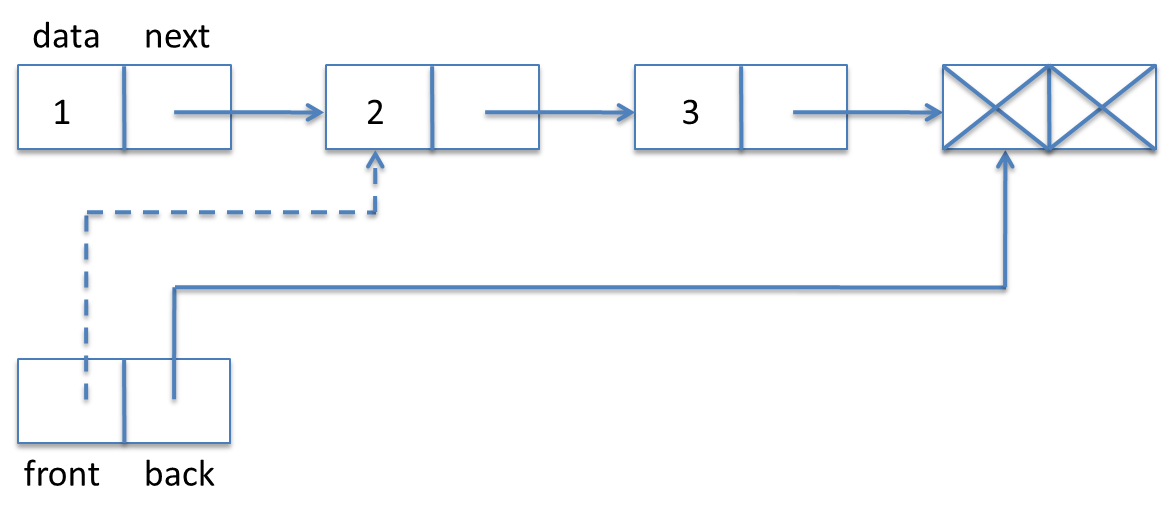
\includegraphics[width=0.85\textwidth]{img/queue4.png}
\end{center}
And in code:
\begin{lstlisting}[language={[C0]C}]
elem deq(queue* Q)
//@requires is_queue(Q);
//@requires !queue_empty(Q);
//@ensures is_queue(Q);
{
  elem x = Q->front->data;
  Q->front = Q->front->next;
  return x;
}
\end{lstlisting}

\clearpage
\noindent
Let's verify that our pointer dereferencing operations are safe.  We
have
\begin{lstlisting}[language={[C0]C}]
  Q->front->data
\end{lstlisting}
which entails two pointer dereference.  We know \lstinline'is_queue(Q)'
from the precondition of the function.  Recall:
\begin{lstlisting}[language={[C0]C}]
bool is_queue(queue Q) {
  return Q != NULL
      && is_acyclic(Q->front)
      && is_segment(Q->front, Q->back);
}
\end{lstlisting}
We see that \lstinline'Q->front' is okay, because by the first
test we know that \lstinline'Q != NULL' is the precondition holds.
By the second test we see that both \lstinline'Q->front'
and \lstinline'Q->back' are not null, and we can therefore
dereference them.

We also make the assignment \lstinline'Q->front = Q->front->next'.  Why
does this preserve the invariant?  Because we know that the queue is
not empty (second precondition of \lstinline'deq') and therefore
\lstinline'Q->front != Q->back'.  Because \lstinline'Q->front' to \lstinline'Q->back'
is a valid non-empty segment, \lstinline'Q->front->next' cannot be null.

An interesting point about the dequeue operation is that we do not
explicitly deallocate the first element.  If the interface is
respected there cannot be another pointer to the item at the front of
the queue, so it becomes \emph{unreachable}: no operation of the
remainder of the running programming could ever refer to it.  This
means that the garbage collector of the C0 runtime system will recycle
this list item when it runs short of space.


\section{Stacks with Linked Lists}
\label{sec:linkedlist:stacks}
\TAGS{correctness, ds-invariant, linked-list, safety, stack}

For the implementation of stacks, we can reuse linked lists and the
basic structure of our queue implementation, except that we read off
elements from the same end that we write them to. We call the pointer
to this end \lstinline'top'. Since we do not perform operations on the
other side of the stack, we do not necessarily need a pointer to the
other end.  For structural reasons, and in order to identify the
similarities with the queue implementation, we still decide to
remember a pointer \lstinline'floor' to a dummy node right after the
last element (or \emph{bottom}) of the stack.  With
this design decision, the validation function \lstinline'is_stack',
internal to the library implementation, and the client operations
\lstinline'stack_empty' and \lstinline'stack_new' are implemented
identically to what we saw for queues.  The \lstinline'floor' pointer
of the stack is otherwise unused.  A typical stack then has the
following form:
\begin{center}
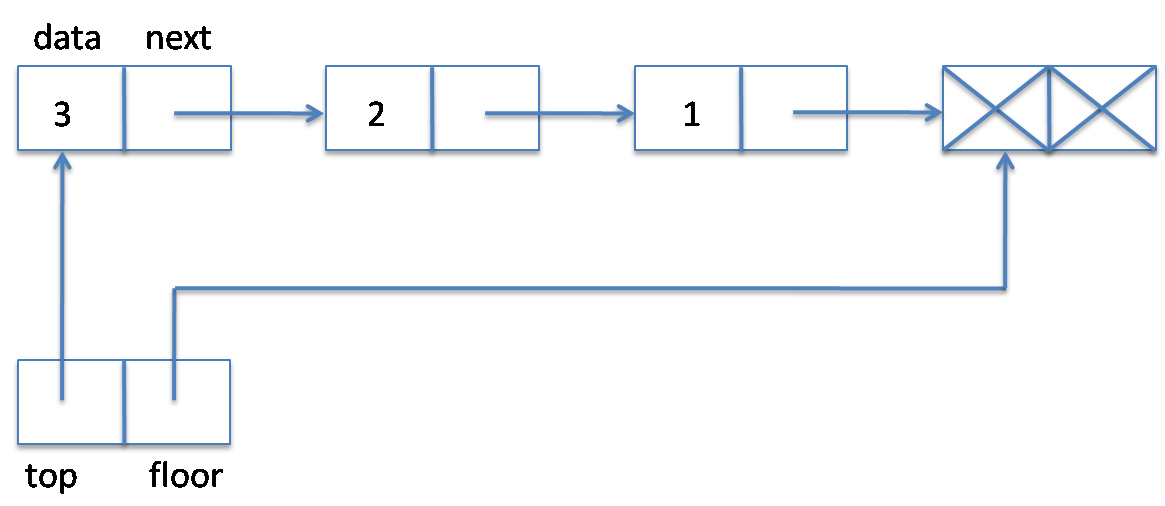
\includegraphics[width=0.85\textwidth]{img/stack1.png}
\end{center}
Here, $3$ is the element at the top of the stack.

We define:
\begin{lstlisting}[language={[C0]C}]
typedef struct stack_header stack;
struct stack_header {
  list* top;
  list* floor;
};

bool is_stack(stack* S) {
  return S != NULL
      && is_acyclic(S->top)
      && is_segment(S->top, S->floor);
}
\end{lstlisting}

Popping from a stack requires taking an item from the front of the
linked list, which is much like dequeuing.
\begin{lstlisting}[language={[C0]C}]
elem pop(stack* S)
//@requires is_stack(S);
//@requires !stack_empty(S);
//@ensures is_stack(S);
{
  elem x = S->top->data;
  S->top = S->top->next;
  return x;
}
\end{lstlisting}

To push an element onto the stack, we create a new list item, set its
data field and then its next field to the current top of the stack ---
the opposite end of the linked list from the queue.
Finally, we need to update the \lstinline'top' field of the stack to point
to the new list item.  While this is simple, it is still a good idea
to draw a diagram.  We go from
\begin{center}
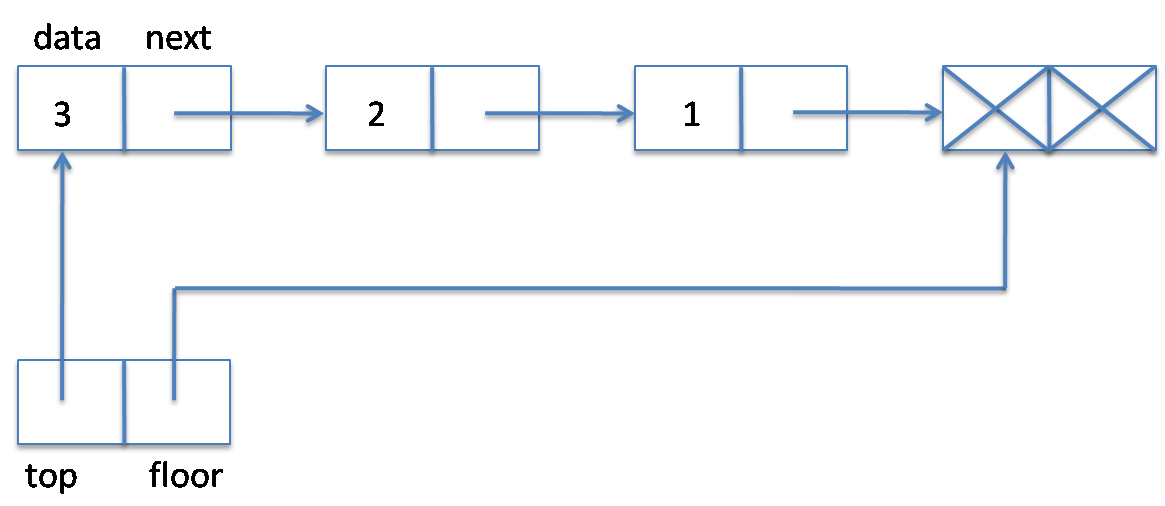
\includegraphics[width=0.8\textwidth]{img/stack1.png}
\end{center}
to
\begin{center}
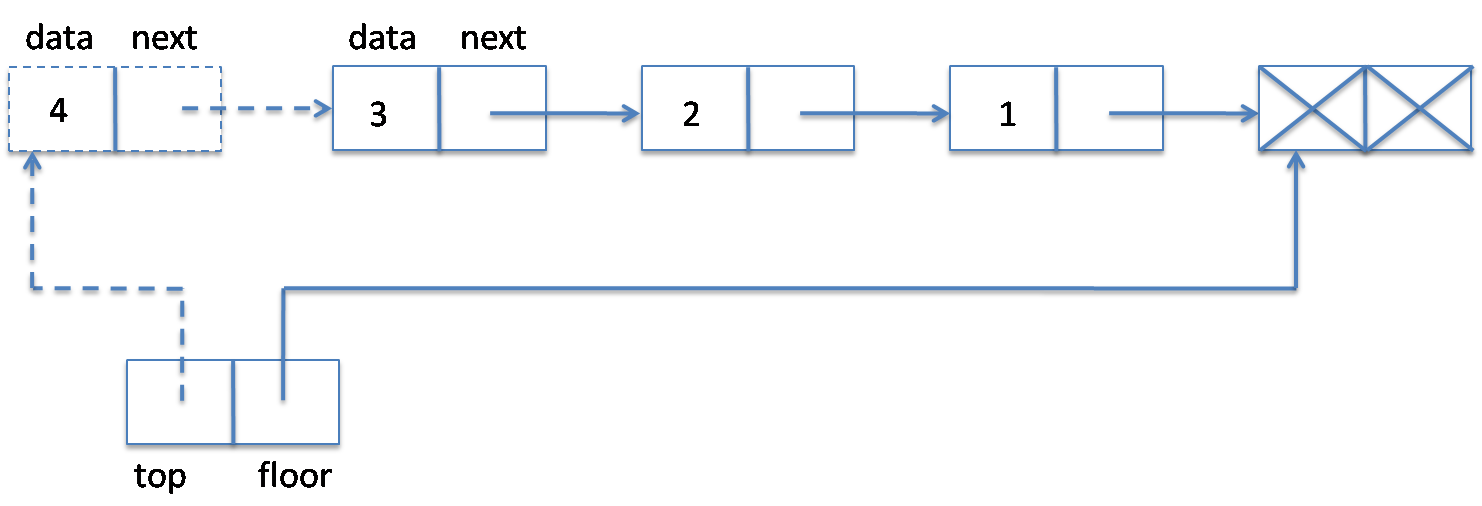
\includegraphics[width=0.99\textwidth]{img/stack2.png}
\end{center}
In code:
\begin{lstlisting}[language={[C0]C}]
void push(stack* S, elem x)
//@requires is_stack(S);
//@ensures is_stack(S);
{
  list* p = alloc(list);  // Allocate a new top node
  p->data = x;
  p->next = S->top;
  S->top = p;
}
\end{lstlisting}

The client-side type \lstinline'stack_t' is defined as a pointer to a
\lstinline'stack_header':
\begin{lstlisting}[language={[C0]C}]
typedef stack* stack_t;
\end{lstlisting}

\noindent
This completes the implementation of stacks.


\section{Sharing}
\label{sec:linkedlist:sharing}
\TAGS{aliasing, correctness, linked-list, safety}

We observed in the last section that the \lstinline'floor' pointer of
a \lstinline'stack_header' structure is unused other than for checking
that a stack is empty.  This suggests a simpler representation, where
we take the empty stack to be \lstinline'NULL' and do without the
\lstinline'floor' pointer.  This yields the following declarations
\begin{lstlisting}[language={[C0]C}]
typedef struct stack_header stack;
struct stack_header {
  list* top;
};

bool is_stack(stack* S) {
  return S != NULL && is_acyclic(S->top);
}
\end{lstlisting}
and pictorial representation of a stack:
\begin{center}
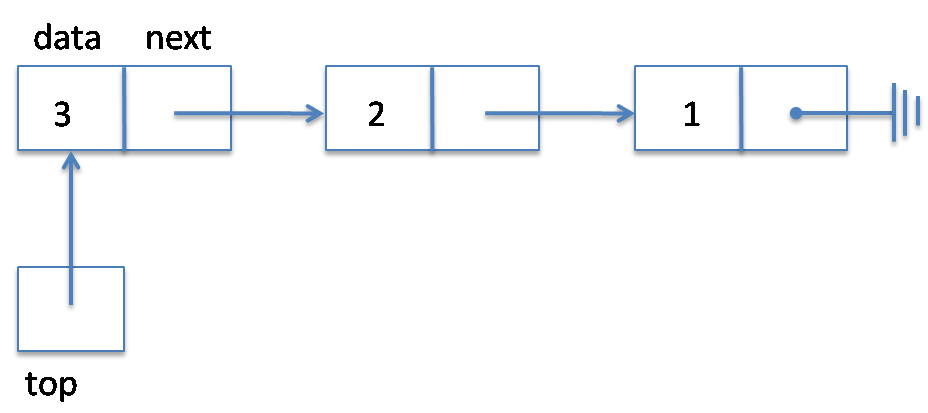
\includegraphics[width=0.65\textwidth]{img/stackB.png}
\end{center}
But, then, why have a header at all?  Can't we define the stack simply
to be the linked list pointed by \lstinline'top' instead?

Eliminating the header would lead to a redesign of the interface and
therefore to changes in the code that the client writes.
Specifically,
\begin{enumerate}
\item%
  \lstinline'NULL' is now a valid stack --- it represents the empty
  stack.  Therefore, we would have to remove all those
  \lstinline'NULL' checks from the interface.  (Alternatively, we
  can bring back the dummy node, but this time with a mandatory
  \lstinline'NULL' pointer in the \lstinline'next' field.)
\item%
  More dramatically, we need to change the type of \lstinline'push'
  and \lstinline'pop'.  Consider performing the operation
  \lstinline'push(S, 4)' where \lstinline'S' contains the address of
  the stack from the caller's perspective:
  \begin{center}
    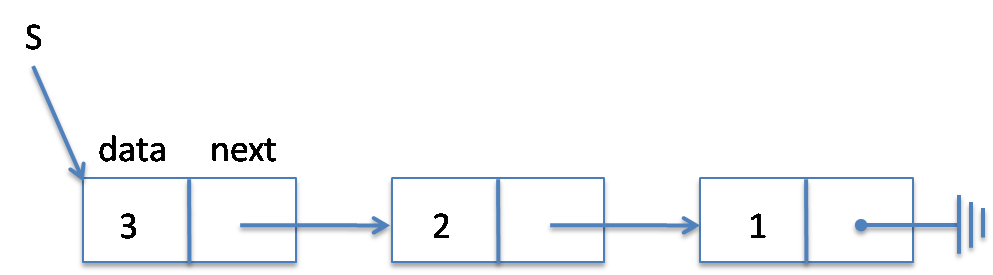
\includegraphics[width=0.65\textwidth]{img/stackC.png}
  \end{center}
  This call would result in the following stack:
  \begin{center}
    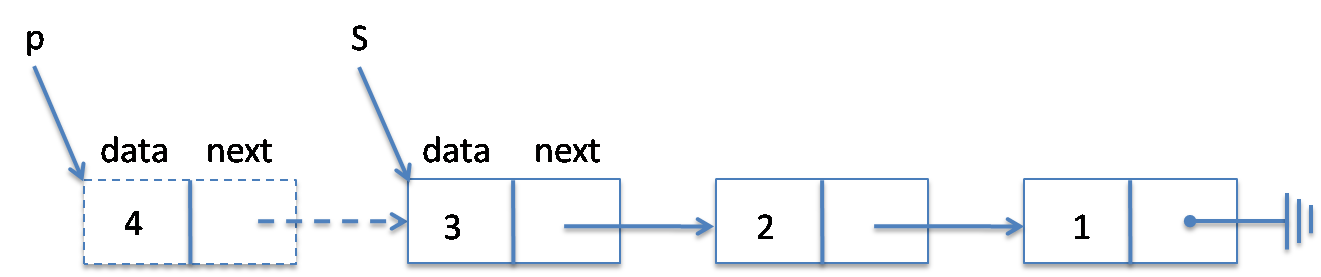
\includegraphics[width=0.85\textwidth]{img/stackC-push.png}
  \end{center}
  where \lstinline'p' is a pointer to the newly allocated list node.
  Note that the stack has not changed from the point of view of the
  caller!  In fact, from the caller's standpoint,  \lstinline'S' still
  points to the node containing 3.  The only way for the caller to
  access the updated stack is that the pointer
  \lstinline'p' be given back to it.  Thus, \lstinline'push' must now
  return the updated stack.  Therefore, we need to change its
  prototype to
\begin{lstlisting}[language={[C0]C}]
stack_t push(stack_t S, elem x);
\end{lstlisting}
  The same holds for \lstinline'pop', with a twist: \lstinline'pop'
  already returns the value at the top of the stack.  It now needs to
  return both this value and the updated stack.
\end{enumerate}
With such header-less stacks, the client has the illusion that
\lstinline'push' and \lstinline'pop' produces a new stack each time
they are invoked.  However, the underlying linked lists share many of
the same elements.  Consider performing the following operations on the
stack \lstinline'S' above:
\begin{lstlisting}[language={[C0]C}]
stack_t S1 = push(S, 4);
stack_t S2 = push(S, 5);
\end{lstlisting}
This yields the following memory layout:
\begin{center}
  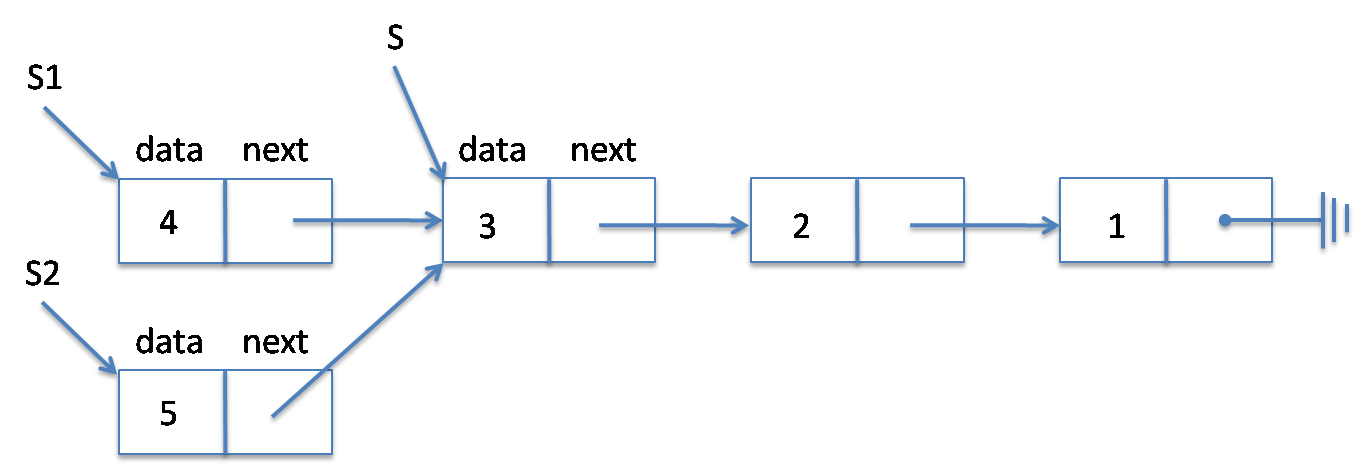
\includegraphics[width=0.9\textwidth]{img/stackC-push2.png}
\end{center}
All three stacks share nodes 3, 2 and 1.  Observe furthermore that the
second call to \lstinline'push' operated on \lstinline'S', which
remained unchanged after the first call.  At this point, a
\lstinline'pop' on \lstinline'S' would result in a fourth stack, say
\lstinline'S3', which points to node 2.

Sharing is an efficient approach to maintaining multiple versions of a
data structure as a sequence of operations is performed on them.
Sharing is not without its perils, however.  As an exercise, consider
an implementation of queues such that \lstinline'enq' and
\lstinline'deq' return to their caller a pair of pointers to the front
and back of the underlying linked list (maybe packaged in a
\lstinline'struct').  A carefully chosen series of \lstinline'enq' and
\lstinline'deq' operations will break the queue (or more precisely its
representation invariant).


\clearpage
\section{Exercises}
\label{sec:linkedlist:exercises}

\begin{flex}
\begin{exercise}[\opt{sample solution on page~\pageref{ex:linked-list_sum-solved}}]
\label{ex:linked-list_sum}
Define the function
\begin{lstlisting}[language={[C0]C}]
bool is_sum(list* start, list* end, int sum);
\end{lstlisting}
that checks that the sum of all nodes in the segment from
\lstinline'start' to \lstinline'end' is equal to \lstinline'sum'.  You
may assume that the data contained in each node is an integer.  How
should it behave if the segment is empty?
\end{exercise}

\begin{lrbox}{0\null\global\setbox\lstbox}
\begin{lstlisting}[language={[C0]C}]
bool is_sum(list* start, list* end, int sum)
//@requires is_segment(start, end);
{
  list* l = start;
  int n = 0;
  while (l != end) {
    n += l->data;
    l = l-> next;
  }
  return n == sum;
}
\end{lstlisting}
\end{lrbox}

\begin{solution}\opt{\textbf{of exercise~\ref{ex:linked-list_sum}}}
\label{ex:linked-list_sum-solved}
  The sum of all the elements in a list (or
  array) segment would be defined recursively as the first element
  plus the sum of the rest of the segment.  Then, it is natural to
  define the sum of an empty segment to be zero.   Thus,
  \lstinline'is_sum(start, end, n)' on an empty segment would return
  \lstinline'true' exactly when \lstinline'n == 0'.
%% Pulled out in \lstbox to support fancy solutions
% \begin{lstlisting}[language={[C0]C}]
% bool is_sum(list* start, list* end, int sum)
% //@requires is_segment(start, end);
% {
%   list* l = start;
%   int n = 0;
%   while (l != end) {
%     n += l->data;
%     l = l-> next;
%   }
%   return n == sum;
% }
% \end{lstlisting}
\par\medskip\noindent\usebox{\lstbox}\par
\end{solution}
\end{flex}

\begin{lrbox}{0\null\global\setbox\lstbox}
\begin{lstlisting}[language={[C0]C}]
int lseg_len(list* start, list* end)
//@is_segment(start, end);
{
  int n = 0;
  for (list* p = start; p != end; p = p->next)
  //@loop_invariant p != NULL;
  {
    n++;
  }
  return n;
}
\end{lstlisting}
\end{lrbox}

\begin{flex}
\begin{exercise}[\opt{sample solution on page~\pageref{ex:linked-list_length-solved}}]
\label{ex:linked-list_length}
  Define the function
\begin{lstlisting}[language={[C0]C}]
int lseg_len(list* start, list* end)
/*@requires is_segment(start, end); @*/ ;
\end{lstlisting}
that returns the number of elements in the list segment
$[$\lstinline'start',\lstinline'end'$)$.
\end{exercise}

\begin{solution}\opt{\textbf{of exercise~\ref{ex:linked-list_length}}}
\label{ex:linked-list_length-solved}
%% Pulled out in \lstbox to support fancy solutions
% \begin{lstlisting}[language={[C0]C}]
% int lseg_len(list* start, list* end)
% //@is_segment(start, end);
% {
%   int n = 0;
%   for (list* p = start; p != end; p = p->next)
%   //@loop_invariant p != NULL;
%   {
%     n++;
%   }
%   return n;
% }
% \end{lstlisting}
\par\medskip\noindent\usebox{\lstbox}\par
\end{solution}
\end{flex}


\begin{flex}
\begin{exercise}[\opt{sample solution on page~\pageref{ex:linked-list_ith-solved}}]
\label{ex:linked-list_ith}
  Define the function
\begin{lstlisting}
elem ith(list* l, int i)
/*@requires i >= 0; @*/ ;
\end{lstlisting}
that returns the data in \lstinline'i'-th elements in list
\lstinline'l' (counting from 0).  If there are fewer than
\lstinline'i' elements before encountering a \lstinline'NULL' pointer,
an assertion should fail.

What is the asymptotic complexity of calling \lstinline'ith(l,i)' on a
list \lstinline'l' with $n$ elements, assuming $0 <= i < n$?
\end{exercise}

\begin{lrbox}{0\null\global\setbox\lstbox}
\begin{lstlisting}[language={[C0]C}]
elem ith(list* l, int i)
//@requires i >= 0;
{
  for (list* p = l; p != NULL; p = p->next) {
    if (i == 0) return p->data;
    i--;
  }
  assert(false);   // i is greater than the length of l
  return p->data;  // possibly unsafe but unreachable
}
\end{lstlisting}
\end{lrbox}

\begin{solution}\opt{\textbf{of exercise~\ref{ex:linked-list_ith}}}
\label{ex:linked-list_ith-solved}
%% Pulled out in \lstbox to support fancy solutions
% \begin{lstlisting}[language={[C0]C}]
% elem ith(list* l, int i)
% //@requires i >= 0;
% {
%   for (list* p = l; p != NULL; p = p->next) {
%     if (i == 0) return p->data;
%     i--;
%   }
%   assert false;  // i is greater than the length of l
% }
% \end{lstlisting}
\par\medskip\noindent\usebox{\lstbox}\par
For an $n$-element list \lstinline'l', the asymptotic complexity of
\lstinline'ith(l,i)' is $O(n)$.
\end{solution}
\end{flex}


\begin{flex}
\begin{exercise}[\opt{sample solution on page~\pageref{ex:linked-list-util-solved}}]
\label{ex:linked-list-util}
Define the following specification functions on list segments with
integer elements:
\begin{lstlisting}[language={[C0]C}]
bool is_in_lseg(int x, list* start, list* end)
/*@requires is_segment(start, end); @*/ ;
bool is_sorted_lseg(list* start, list* end)
/*@requires is_segment(start, end); @*/ ;
\end{lstlisting}
The first returns \lstinline'true' if \lstinline'x' occurs in the list
segment $[$\lstinline'start'$,$\lstinline'end'$)$ and \lstinline'false'
otherwise.  The second returns \lstinline'true' if the input list
segment is sorted in ascending order.
\end{exercise}

\begin{lrbox}{0\null\global\setbox\lstbox}
\begin{lstlisting}[language={[C0]C}]
bool is_in_lseg(int x, list* start, list* end)
//@requires is_segment(start, end);
{
  for (list* p = start; p != end; p = p->next)
  //@loop_invariant p != NULL;
  {
    if (p->data == x) return true;
  }
  return false;
}

bool is_sorted_lseg(list* start, list* end)
//@requires is_segment(start, end);
{
  if (start == end)  // empty list segment
    return true;

  int x = start->data;
  for (list* p = start->next; p != end; p = p->next)
  //@loop_invariant p != NULL;
  {
    if (x > p->data) return false;
    x = p->data;
  }
  return true;
}
\end{lstlisting}
\end{lrbox}

\begin{solution}\opt{\textbf{of exercise~\ref{ex:linked-list-util}}}
\label{ex:linked-list-util-solved}
%% Pulled out in \lstbox to support fancy solutions
% \begin{lstlisting}[language={[C0]C}]
% bool is_in_lseg(int x, list* start, list* end)
% //@requires is_segment(start, end);
% {
%   for (list* p = start; p != end; p = p->next)
%   //@loop_invariant p != NULL;
%   {
%     if (p->data == x) return true;
%   }
%   return false;
% }

% bool is_sorted_lseg(list* start, list* end)
% //@requires is_segment(start, end);
% {
%   if (start == end)  // empty list segment
%     return true;

%   int x = start->data;
%   for (list* p = start->next; p != end; p = p->next)
%   //@loop_invariant p != NULL;
%   {
%     if (x > p->data) return false;
%     x = p->data;
%   }
%   return true;
% }
% \end{lstlisting}
\par\medskip\noindent\usebox{\lstbox}\par
\end{solution}
\end{flex}


\begin{flex}
\begin{exercise}[\opt{sample solution on page~\pageref{ex:linked-list-binsearch-solved}}]
\label{ex:linked-list-binsearch}
  The function \lstinline'ith(l,i)' you defined in an earlier exercise
  works just like an array access \lstinline'A[i]', except that it
  does so on a linked list.  Using it and other functions you wrote
  for previous exercises, implement a version of binary search that
  operates on list segments.  For simplicity, you may assume that the
  type \lstinline'elem' of data elements has been defined to be
  \lstinline'int'.  Here's the function prototype.
\begin{lstlisting}[language={[C0]C}]
int lseg_binsearch(int x, list* start, list* end)
//@requires is_segment(start, end);
//@requires is_sorted_lseg(l, start, end);
/*@ensures (\result == -1 || !is_in_lseg(x, start, end))
        || (0 < \result && \result < lseg_len(start, end) &&
            ith(start, \result) == x);
@*/ ;
\end{lstlisting}

What is the asymptotic complexity of calling
\lstinline'lseg_binsearch(x,start,end)' on a list segment
$[$\lstinline'start'$,$ \lstinline'end'$)$ with $n$ elements?
\end{exercise}

\begin{lrbox}{0\null\global\setbox\lstbox}
\begin{lstlisting}[language={[C0]C}]
int lseg_binsearch(int x, list* start, list* end)
//@requires is_sorted_lseg(A, 0, n);
/*@ensures (\result == -1 || !is_in_lseg(x, start, end))
        || (0 < \result && \result < lseg_len(start, end) &&
            \ith(start, \result) == x); @*/
{
  int lo = 0;
  int hi = lseg_len(start, end);

  while (lo < hi)
  //@loop_invariant 0 <= lo && lo <= hi && hi <= n;
  {
    int mid = lo + (hi - lo)/2;
    //@assert lo <= mid && mid < hi;

    int mid_data = ith(start, mid);
    if (mid_data == x) return mid;
    if (mid_data < x) {
      lo = mid+1;
    } else { //@assert mid_data > x;
      hi = mid;
    }
  }
  //@assert !is_in_lseg(x,start,end);
  return -1;
}
\end{lstlisting}
\end{lrbox}

\begin{solution}\opt{\textbf{of exercise~\ref{ex:linked-list-binsearch}}}
\label{ex:linked-list-binsearch-solved}
%% Pulled out in \lstbox to support fancy solutions
% \begin{lstlisting}[language={[C0]C}]
% int lseg_binsearch(int x, list* start, list* end)
% //@requires is_sorted_lseg(A, 0, n);
% /*@ensures (\result == -1 || !is_in_lseg(x, start, end))
%         || (0 < \result && \result < lseg_len(start, end) &&
%             \ith(start, \result) == x); @*/
% {
%   int lo = 0;
%   int hi = lseg_len(start, end);

%   while (lo < hi)
%   //@loop_invariant 0 <= lo && lo <= hi && hi <= n;
%   {
%     int mid = lo + (hi - lo)/2;
%     //@assert lo <= mid && mid < hi;

%     int mid_data = ith(start, mid);
%     if (mid_data == x) return mid;
%     if (mid_data < x) {
%       lo = mid+1;
%     } else { //@assert mid_data > x;
%       hi = mid;
%     }
%   }
%   //@assert !is_in_lseg(x,start,end);
%   return -1;
% }
% \end{lstlisting}
\par\medskip\noindent\usebox{\lstbox}\par
The complexity of \lstinline'lseg_binsearch' is $O(n \log n)$: it will
make $\log n$ accesses to the list (just like binary search) but each
access now costs $O(n)$.
\end{solution}
\end{flex}


\begin{exercise}
  The tortoise-and-hare implementation of circularity checking we gave
  has an assertion, \lstinline't != NULL', which we can't prove with
  the given loop invariants. What loop invariants would allow us to
  prove that assertion correct? Can we write loop invariants that
  allow us to prove, when the loop exits, that we have found a cycle?
\end{exercise}

\begin{exercise}
  Consider what would happen if we \lstinline'pop' an element from the
  empty stack when contracts are not checked in the linked list
  implementation?  When does an error arise?
\end{exercise}

\begin{exercise}
  Complete the implementations of stack as defined at the beginning of
  Section~\ref{sec:linkedlist:sharing}, dispensing with the
  \lstinline'floor' pointer, terminating the list with
  \lstinline'NULL' instead.
\end{exercise}

\begin{exercise}
  Consider an implementation of queues as linked list such that
  \lstinline'enq' and \lstinline'deq' return to their caller a new
  header to the front and back of the underlying linked list each time
  they are called.  Engineer a series of \lstinline'enq' and
  \lstinline'deq' operations that, starting from a valid queue, will
  result in a data structure that does not satisfy the representation
  invariant of queues (i.e., result in a broken queue).
\end{exercise}


\begin{flex}
\begin{exercise}[\opt{sample solution on page~\pageref{ex:linked-list_bad-is_acyclic-solved}}]
\label{ex:linked-list_bad-is_acyclic}
  Here's a simple idea to check that a linked list is acyclic: first,
  we make a copy \lstinline'p' of the \lstinline'start' pointer.  Then
  when we advance \lstinline'p' we run through an auxiliary loop to
  check if its next element is already in the list.  The code would be
  something like this:
\begin{lstlisting}[language={[C0]C}]
bool is_acyclic(list* start) {
  for (list* p = start; p != NULL; p = p->next)
  //@loop_invariant is_segment(start, p);
  {
    if (p == NULL) return true;

    for (list* q = start; q != p; q = q->next)
    //@loop_invariant is_segment(start, q);
    //@loop_invariant is_segment(q, p);
    {
      if (q == p->next) return false; /* circular */
    }
  }
  return true;
}
\end{lstlisting}
  This code has however an issue.  Can you find it?
\end{exercise}

\begin{lrbox}{0\null\global\setbox\lstbox}
\begin{lstlisting}[language={[C0]C}]
int main() {
  list* a = alloc(list);
  a->next = a;                         // self loop
  assert(is_acyclic(a, NULL));
  return 0;
}
\end{lstlisting}
\end{lrbox}

\begin{solution}\opt{\textbf{of exercise~\ref{ex:linked-list_bad-is_acyclic}}}
\label{ex:linked-list_bad-is_acyclic-solved}
The code does not work when the input-list is a self-loop, as in the
following example:
%% Pulled out in \lstbox to support fancy solutions
% \begin{lstlisting}[language={[C0]C}]
% int main() {
%   list* a = alloc(list);
%   a->next = a;                         // self loop
%   assert(is_acyclic(a, NULL));
%   return 0;
% }
% \end{lstlisting}
\par\medskip\noindent\usebox{\lstbox}\par
\end{solution}
\end{flex}


\begin{exercise}
We say ``on the \emph{i\textsuperscript{th}} iteration of our naive
\lstinline'is_segment' loop, we know that we can get from \lstinline'start' to
\lstinline'p' by following exactly $i$ pointers.'' Write a function
\lstinline'is_reachable_in(list* start, list* end, int numsteps)'; this
function should
return \lstinline'true' if we can get from \lstinline'start' to \lstinline'end' in
exactly \lstinline'numsteps' steps. Use this function as a loop invariant for
\lstinline'is_segment'.
\end{exercise}

\begin{exercise}
  What happens when we swap the order of the lines in the \lstinline'enq'
  function and why?
\end{exercise}

\begin{exercise}
  Write an interface and implementation of a \emph{double-ended queue}
  where we can add and remove elements at both ends.  Make sure that
  all operations you specify can be implemented in constant time.
\end{exercise}



\printsolutions
% \clearpage
% \bibliographystyle{alpha}
% \bibliography{modal}




% \begin{comment}
% \newpage
% \section{Checking for circularity (The bounded reachability way)}
% \label{sec:linkedlist:bounded_reachability}

% In lecture we developed a
% reasonable way of checking for circularity. The idea that is implicit
% in the solution we discovered is that, if you have a circular linked
% list structure, then eventually you are going encounter a node that
% you've seen before. So what we need is an always-terminating way of
% checking all the places we've already seen.

% A helper function that can be useful for this operation is one that
% we'll call \lstinline'is_in_bounded(x, start, n)'. This function tells us
% whether we'll get to the list node \lstinline'x' from \lstinline'start' by
% following no more than \lstinline'n' pointers.

% \begin{lstlisting}[language={[C0]C}]
% bool is_in_bounded(list* x, list* start, int numsteps)
% //@requires 0 <= numsteps;
% {
%   int i = 0;
%   for (list* p = start; p != NULL; p = p->next)
%     //@loop_invariant 0 <= i && i <= numsteps;
%     {
%       if (i == numsteps) {
%         // If the thing we're looking for is in the list,
%         // it is further on.
%         return false;
%       }

%       if (p == x) {
%         // Oh, here it is!
%         return true;
%       }

%       i += 1;
%     }

%   // We reached a NULL, it's not in the bounded list
%   return false;
% }
% \end{lstlisting}

% \newpage
% On the $i$\textsuperscript{th} iteration of our naive \lstinline'is_segment'
% loop, we know that we can get from \lstinline'start' to \lstinline'p' by
% following exactly $i$ pointers. We know we have a cycle if we can
% \emph{also} get \lstinline'p' by following \emph{fewer} than $i$ pointers.
% In our example of a circular linked list, we could get to the list
% node containing $7$ by following either $1$ \lstinline'next' pointer or $4$
% \lstinline'next' pointers, and we will return \lstinline'false' the second time
% we encounter that node.

% \begin{lstlisting}[language={[C0]C}]
% // Always returns true or false
% bool is_segment(list* start, list* end) {
%   int i = 0;
%   for (list* p = start; p != NULL; p = p->next)
%     //@loop_invariant 0 <= i;
%     {
%       //@assert(is_in_bounded(p, start, i+1));
%       if (is_in_bounded(p, start, i)) return false; // CYCLE!
%       if (p == end) return true; // DONE!
%       i += 1;
%     }

%   // We reached NULL without getting to end first
%   return false;
% }
% \end{lstlisting}


% \section{Plain Linked Lists}
% \label{sec:linkedlist:null_termination}

% Later in this course, we will occasionally embed linked lists within
% data structures, subject to the only requirement that they be acyclic.
% These lists will have an obvious front and we will use
% \lstinline'NULL' as an end-of-list marker --- we will have no use for
% a dummy node or a pointer to the back.  Building on the code developed
% so far, a representation invariant for such lists is simply:
% \begin{lstlisting}
% bool is_list(list* l) {
%   return is_acyclic(l, NULL);
% }
% \end{lstlisting}

% \end{comment}
